% Generated by pysimcount.pfseeds -- do not edit; regenerate instead.
% figure: A-measured-by-order -- Suzuki formulas of each order, r from: Measured $r$; median over seeds [1, 2, 3, 4, 5, 6, 7, 8, 9, 10], bars = min..max
% metric=total gatebase=cz merged
% seed 1: git_commit=01d3c275ceae2840002bd1aaea68f59b987c4975 git_dirty=False
% seed 2: git_commit=01d3c275ceae2840002bd1aaea68f59b987c4975 git_dirty=False
% seed 3: git_commit=01d3c275ceae2840002bd1aaea68f59b987c4975 git_dirty=False
% seed 4: git_commit=01d3c275ceae2840002bd1aaea68f59b987c4975 git_dirty=False
% seed 5: git_commit=01d3c275ceae2840002bd1aaea68f59b987c4975 git_dirty=False
% seed 6: git_commit=01d3c275ceae2840002bd1aaea68f59b987c4975 git_dirty=False
% seed 7: git_commit=01d3c275ceae2840002bd1aaea68f59b987c4975 git_dirty=False
% seed 8: git_commit=01d3c275ceae2840002bd1aaea68f59b987c4975 git_dirty=False
% seed 9: git_commit=01d3c275ceae2840002bd1aaea68f59b987c4975 git_dirty=False
% seed 10: git_commit=01d3c275ceae2840002bd1aaea68f59b987c4975 git_dirty=False
% derived: A-measured-by-order.tex with Lie-Trotter S1 removed by pysimcount.figdrop (Lie-Trotter S1 alone spans 45% of the original y-axis); removed legends: Lie-Trotter S1; source_sha256=e2bf84ffb599868fe2a49247c1a07a142bbb247e7fcbcfa12855e9fbdd5d40d5
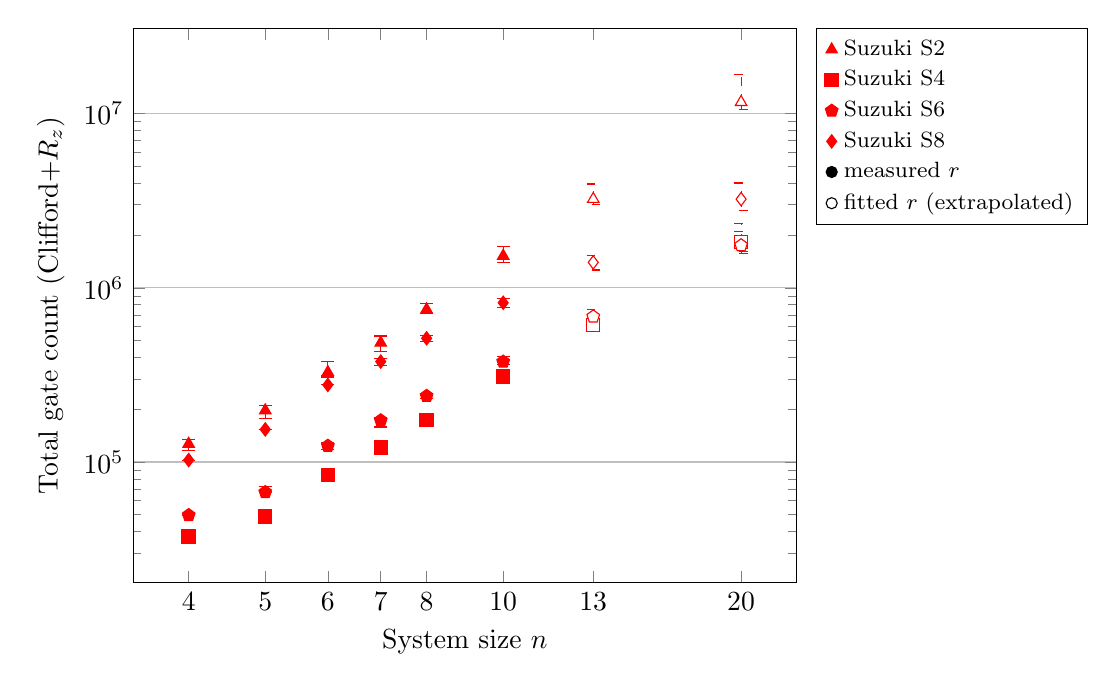
\begin{tikzpicture}
  \begin{loglogaxis}[
    width=10cm,
    xlabel={System size $n$},
    ylabel={Total gate count (Clifford+$R_z$)},
    xtick={4,5,6,7,8,10,13,20},
    xticklabels={4,5,6,7,8,10,13,20},
    ymajorgrids=true,
    legend pos=outer north east,
    legend cell align=left,
    legend style={font=\footnotesize},
  ]
    \addplot[only marks, red, mark=triangle*, mark size=2.4pt, mark options={solid, fill=red}, error bars/.cd, y dir=both, y explicit, error bar style={red}] coordinates {
      (4,127008) += (0,7200) -= (0,11040)
      (5,197760) += (0,13200) -= (0,20400)
      (6,327600) += (0,49104) -= (0,15120)
      (7,483672) += (0,45864) -= (0,52584)
      (8,750912) += (0,64320) -= (0,40128)
      (10,1524720) += (0,208080) -= (0,126960)
    };
    \addlegendentry{Suzuki S2}
    \addplot[only marks, red, mark=triangle*, mark size=2.4pt, mark options={solid, fill=white}, forget plot, error bars/.cd, y dir=both, y explicit, error bar style={red, dashed}] coordinates {
      (13,3234192) += (0,718224) -= (0,222768)
      (20,11655360) += (0,5156160) -= (0,1104000)
    };
    \addplot[only marks, red, mark=square*, mark size=2.4pt, mark options={solid, fill=red}, error bars/.cd, y dir=both, y explicit, error bar style={red}] coordinates {
      (4,37312) += (0,848) -= (0,0)
      (5,48760) += (0,2120) -= (0,1060)
      (6,83952) += (0,6360) -= (0,3816)
      (7,120946) += (0,11130) -= (0,6678)
      (8,174688) += (0,6784) -= (0,6784)
      (10,310580) += (0,28620) -= (0,7420)
    };
    \addlegendentry{Suzuki S4}
    \addplot[only marks, red, mark=square*, mark size=2.4pt, mark options={solid, fill=white}, forget plot, error bars/.cd, y dir=both, y explicit, error bar style={red, dashed}] coordinates {
      (13,610454) += (0,86814) -= (0,39962)
      (20,1835920) += (0,517280) -= (0,212000)
    };
    \addplot[only marks, red, mark=pentagon*, mark size=2.4pt, mark options={solid, fill=red}, error bars/.cd, y dir=both, y explicit, error bar style={red}] coordinates {
      (4,49536) += (0,0) -= (0,0)
      (5,67080) += (0,5160) -= (0,0)
      (6,123840) += (0,6192) -= (0,6192)
      (7,173376) += (0,7224) -= (0,14448)
      (8,239424) += (0,8256) -= (0,8256)
      (10,376680) += (0,25800) -= (0,15480)
    };
    \addlegendentry{Suzuki S6}
    \addplot[only marks, red, mark=pentagon*, mark size=2.4pt, mark options={solid, fill=white}, forget plot, error bars/.cd, y dir=both, y explicit, error bar style={red, dashed}] coordinates {
      (13,684216) += (0,67080) -= (0,40248)
      (20,1754400) += (0,350880) -= (0,185760)
    };
    \addplot[only marks, red, mark=diamond*, mark size=2.4pt, mark options={solid, fill=red}, error bars/.cd, y dir=both, y explicit, error bar style={red}] coordinates {
      (4,102640) += (0,0) -= (0,0)
      (5,153960) += (0,0) -= (0,0)
      (6,277128) += (0,30792) -= (0,0)
      (7,377202) += (0,17962) -= (0,17962)
      (8,513200) += (0,20528) -= (0,20528)
      (10,821120) += (0,51320) -= (0,51320)
    };
    \addlegendentry{Suzuki S8}
    \addplot[only marks, red, mark=diamond*, mark size=2.4pt, mark options={solid, fill=white}, forget plot, error bars/.cd, y dir=both, y explicit, error bar style={red, dashed}] coordinates {
      (13,1401036) += (0,133432) -= (0,133432)
      (20,3233160) += (0,769800) -= (0,461880)
    };
    \addlegendimage{only marks, black, mark=*}
    \addlegendentry{measured $r$}
    \addlegendimage{only marks, black, mark=*, mark options={fill=white}}
    \addlegendentry{fitted $r$ (extrapolated)}
  \end{loglogaxis}
\end{tikzpicture}
